\section{Histogrami $P(R)$ v energijskih pasovih}\label{section2}
Skupna gibalna količina v podatkih je bila vedno večja od \SI{500}{\giga\electronvolt}/c
in manjša od \SI{1500}{\giga\electronvolt}/c. Histograme sem najprej risal po energijskih
pasovih zato, da sem lahko preveril legitimnost grafov $M(p_T)$. Graf $P(R)$ zgleda takole:
\begin{figure}[h]
    \begin{center}
        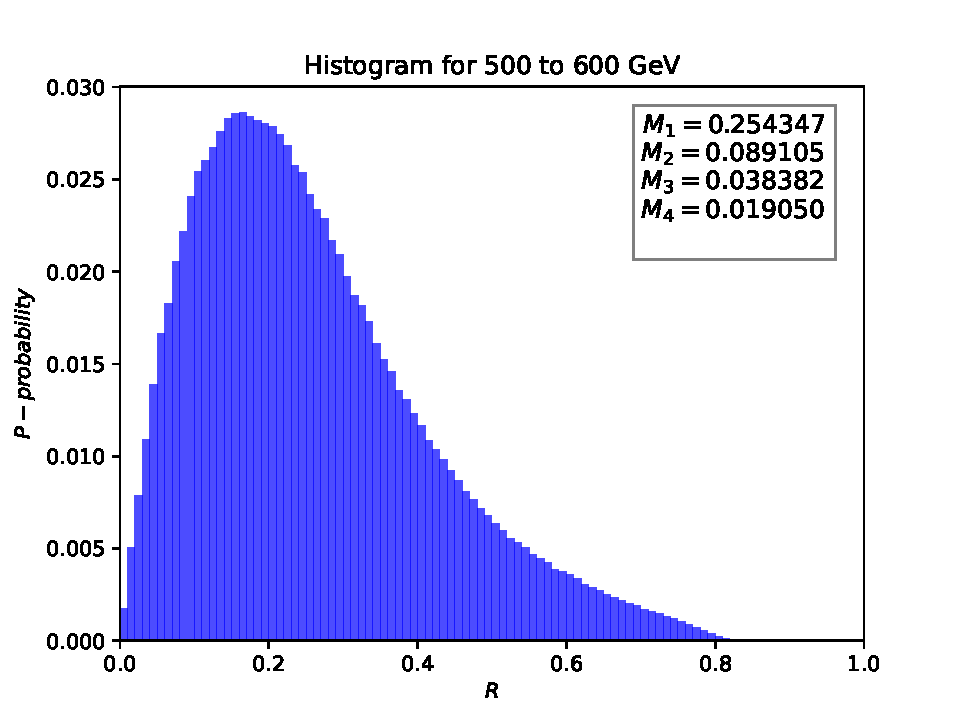
\includegraphics[width=13cm]{sections/section2/figures/1.pdf}
        \caption{Graf $P(R)$ na energijskem pasu 500 do \SI{600}{\giga\electronvolt}/c}
        \label{slika 2}
    \end{center}
\end{figure}
\\
Za definicijo $R$ potrebujemo definirati rapidnost $\eta$ in kot $\phi$. Za rapidnost jeta označimo $\eta_J$ in rapidnost
posameznega delca v jetu $\eta_i$, podobno velja za kot $\phi$. Rapidnost izračunamo
s pomočjo velikosti celotne gibalne količine $p$ in velikosti komponente $p_z$ po tej formuli: 
\begin{equation}
    \eta(p,\,p_z) = \frac{1}{2} \log \left(\frac{p+p_z}{p-p_z}\right) 
\end{equation}
\\
Kot $\phi$ pa je kot med $p_x$ in $p_y$. V sami kodi sem uporabljal funkcijo \verb|numpy.arctan2()|
\begin{equation}
    \phi(p_x, \, p_y) = \arctan\left(\frac{p_x}{p_y}\right)
\end{equation}
Sedaj lahko končno definiramo $R_i$, ki predstavlja $R$ posameznega delca v jetu.
\begin{equation}
    R_i = \left( \left(\eta_J - \eta_i\right)^2 + \left(\phi_J - \phi_i\right)^2 \right)^\frac{1}{2}
\end{equation}
Histogram je bil narisan takole, da je se je vrednost $P$ na intervalu, na katerega je spadal
$R_i$ povečala za $\frac{p_{T_i}}{p_{T_J}N_J}$, kjer $p_T$ označuje transverzalno gibalno količino, 
kjer indeks $i$ predstavlja posamezen delec, indeks $J$ pa celoten jet.
in $N_J$ število jetov. Tak pristop nam zagotovi normaliziran graf. Za vsak graf so bili filtrirani jeti,
ki niso bili v pravem energijskem pasu. 
\\
\\
V grafu so v zgornjem desnem okvirčku izračunani momenti distribuciji. Momenti so definirani takole:
\begin{equation}
    M_i = \sum_{k=0}^{N_b} P(R_k) R_k^i
\end{equation}
Kjer je $N_b$ število intervalov, $k$ pa predstavlja $k$-ti interval.
\\
\\
Koda tega pristopa je v prilogi
pod imenom \verb|R_pt.py|
grafi so pa shranjeni v \verb|i.pdf|, kjer je $i\in\{1,2,3,4,5\}$.
\subsection{Histogrami $P(R^2)$}
Podobno sem narisal distribucije $P(R^2)$, kjer je namesto $R$ argument $R^2$.
Graf izgleda takole:
\begin{figure}[h]
    \begin{center}
        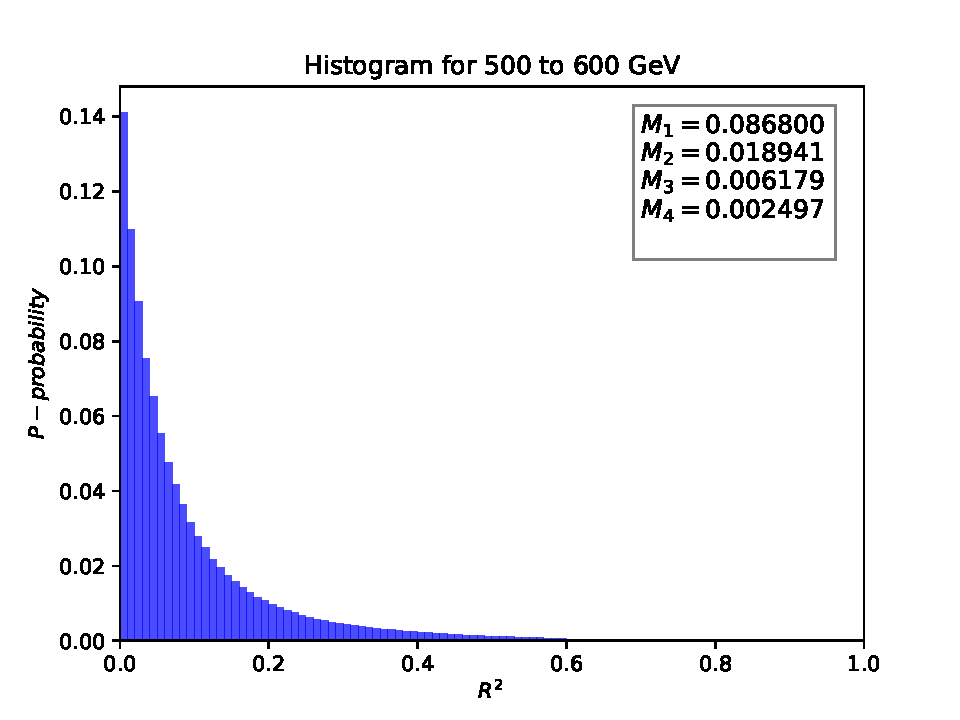
\includegraphics[width=13cm]{sections/section2/figures/1R2.pdf}
        \caption{Graf $P(R^2)$ na energijskem pasu 500 do \SI{600}{\giga\electronvolt}/c}
        \label{slika 3}
    \end{center}
\end{figure}
\\
Nova definicija se glasi:
\begin{equation}
    R_i^2 = \left(\eta_J - \eta_i\right)^2 + \left(\phi_J - \phi_i\right)^2\label{5}
\end{equation}
Grafi so shranjeni v prilogi \verb|iR2.pdf|, kjer je ponovno $i\in\{1,2,3,4,5\}$, koda pa je v
\verb|R2_pt.py|